\documentclass[tikz,border=4pt]{standalone}
\usepackage{tikz}
\usetikzlibrary{patterns,arrows.meta}

% Colors
\definecolor{kmblue}{RGB}{0,56,116}
\definecolor{kmgold}{RGB}{180,140,0}
\definecolor{rtgreen}{RGB}{30,130,60}
\definecolor{servercol}{RGB}{160,60,160}
\definecolor{apcol}{RGB}{200,80,40}
\definecolor{lightgray}{RGB}{220,220,220}

\begin{document}
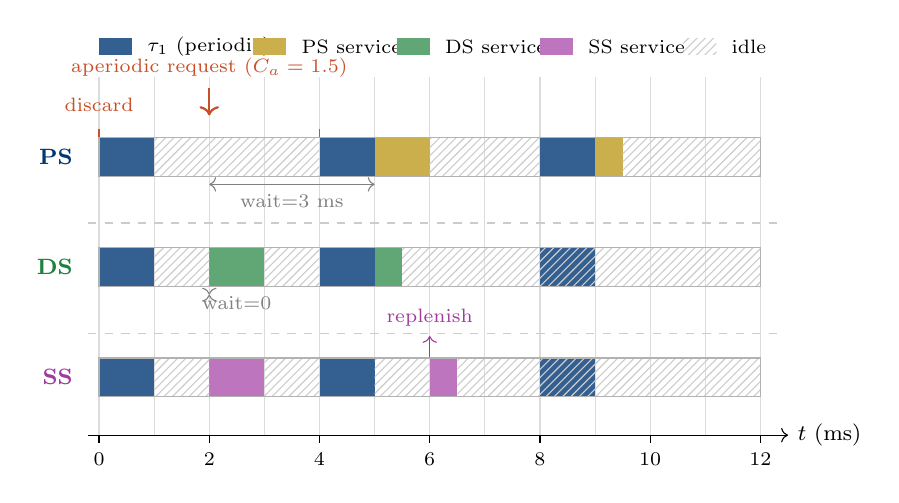
\begin{tikzpicture}[x=0.7cm, y=0.7cm, font=\small]

% ---- layout constants ----
% Three rows: PS (y=5), DS (y=3), SS (y=1)
% Timeline 0..12
% Task τ1 (C=1,T=4): jobs at 0,4,8
% Aperiodic request arrives at t=2, C=1.5
% Server budget Bs=1, Ts=4 for PS/DS; Ss uses replenishment

\def\xscale{0.7}  % already baked into x=0.7cm

% ---- Background grid ----
\foreach \t in {0,1,...,12} {
  \draw[lightgray, thin] (\t,0.3) -- (\t,6.8);
}

% ---- Time axis ----
\draw[->] (-0.2,0.3) -- (12.5,0.3) node[right]{\footnotesize $t$ (ms)};
\foreach \t in {0,2,4,6,8,10,12} {
  \draw (\t,0.3) -- (\t,0.15) node[below,font=\scriptsize]{\t};
}

% ---- Row labels ----
\node[left, font=\footnotesize\bfseries, text=kmblue] at (-0.3,5.35) {PS};
\node[left, font=\footnotesize\bfseries, text=rtgreen] at (-0.3,3.35) {DS};
\node[left, font=\footnotesize\bfseries, text=servercol] at (-0.3,1.35) {SS};

% Row separators
\draw[gray!40,dashed] (-0.2,2.15) -- (12.3,2.15);
\draw[gray!40,dashed] (-0.2,4.15) -- (12.3,4.15);

% ---- Aperiodic request arrow ----
\draw[->, thick, apcol] (2,6.6) -- (2,6.1)
  node[above, at start, font=\scriptsize, apcol]{aperiodic request ($C_a=1.5$)};

% ===== POLLING SERVER (y base = 5) =====
% Server budget Bs=1, replenishes at period boundaries 0,4,8
% PS discards unused budget at replenishment point
% τ1 jobs: [0,1],[4,5],[8,9]  (prio higher than server)
% Server budget available: [0,4)→1 unit; [4,8)→1 unit; [8,12)→1 unit
% τ1 runs: [0,1],[4,5],[8,9]
% Server polls at t=0: no aperiodic yet → budget discarded at t=0 end (nothing to serve)
% Aperiodic arrives t=2. Next PS replenishment t=4.
%   At t=4: τ1 runs [4,5], then PS gets budget=1: serves aperiodic [5,6], remaining 0.5 lost
%   Still 0.5 aperiodic left. Next budget at t=8: τ1 [8,9], PS serves [9,9.5]
% Wait time: arrives t=2, first service t=5 → wait = 3

% τ1 (blue)
\fill[kmblue!80] (0,5) rectangle (1,5.7);
\fill[kmblue!80] (4,5) rectangle (5,5.7);
\fill[kmblue!80] (8,5) rectangle (9,5.7);

% PS server service (purple): [5,6] and [9,9.5]
\fill[kmgold!70] (5,5) rectangle (6,5.7);
\fill[kmgold!70] (9,5) rectangle (9.5,5.7);

% Idle / waiting hatched
\fill[pattern=north east lines, pattern color=gray!40] (1,5) rectangle (4,5.7);
\fill[pattern=north east lines, pattern color=gray!40] (6,5) rectangle (8,5.7);
\fill[pattern=north east lines, pattern color=gray!40] (9.5,5) rectangle (12,5.7);

% budget discarded marker at t=0 (no request yet)
\draw[apcol, dashed, thin] (0,5.7) -- (0,6.0) node[above,font=\scriptsize,apcol]{discard};
\draw[apcol, dashed, thin] (4,5.7) -- (4,6.0);

% wait brace for PS
\draw[<->, gray] (2,4.85) -- (5,4.85) node[midway,below,font=\scriptsize]{wait=3 ms};

% ===== DEFERRABLE SERVER (y base = 3) =====
% DS holds budget; aperiodic at t=2 served immediately with remaining budget
% Budget Bs=1 replenishes at 0,4,8
% DS budget at t=2: still 1 (τ1 has higher prio so DS ran [0,0] effectively, budget=1)
% Actually τ1 runs [0,1] first (higher prio). Then DS has budget=1 at t=1.
% Aperiodic arrives t=2. DS still has budget=1. Serves [2,3]. Remaining=0.5 waits for t=4 replenish.
% At t=4: τ1 [4,5], DS gets budget=1, serves remaining 0.5 at [5,5.5]
% Wait time: 0 (immediate at t=2)

% τ1 (blue)
\fill[kmblue!80] (0,3) rectangle (1,3.7);
\fill[kmblue!80] (4,3) rectangle (5,3.7);
\fill[kmblue!80] (8,3) rectangle (9,3.7);

% DS service (green): [2,3] and [5,5.5]
\fill[rtgreen!70] (2,3) rectangle (3,3.7);
\fill[rtgreen!70] (5,3) rectangle (5.5,3.7);

% idle
\fill[pattern=north east lines, pattern color=gray!40] (1,3) rectangle (2,3.7);
\fill[pattern=north east lines, pattern color=gray!40] (3,3) rectangle (4,3.7);
\fill[pattern=north east lines, pattern color=gray!40] (5.5,3) rectangle (12,3.7);

% wait brace DS
\draw[<->, gray] (2,2.85) -- (2,2.85) ; % zero wait — just a tick
\node[font=\scriptsize, gray] at (2.5,2.7){wait=0};

% ===== SPORADIC SERVER (y base = 1) =====
% SS replenishes on consumption: when budget is consumed, schedule replenishment Ts later
% Initial budget=1 at t=0.
% τ1 [0,1]. Aperiodic arrives t=2. SS budget=1 still. Serves [2,3].
% Replenishment scheduled at t=2+4=6 for 1 unit.
% Remaining 0.5 waits. At t=6, budget=1, serve [6,6.5]. Done.
% Wait=0 for first chunk, gap [3,6] waiting, served at t=6.

% τ1 (blue)
\fill[kmblue!80] (0,1) rectangle (1,1.7);
\fill[kmblue!80] (4,1) rectangle (5,1.7);
\fill[kmblue!80] (8,1) rectangle (9,1.7);

% SS service: [2,3] and [6,6.5]
\fill[servercol!70] (2,1) rectangle (3,1.7);
\fill[servercol!70] (6,1) rectangle (6.5,1.7);

% idle
\fill[pattern=north east lines, pattern color=gray!40] (1,1) rectangle (2,1.7);
\fill[pattern=north east lines, pattern color=gray!40] (3,1) rectangle (4,1.7);
\fill[pattern=north east lines, pattern color=gray!40] (5,1) rectangle (6,1.7);
\fill[pattern=north east lines, pattern color=gray!40] (6.5,1) rectangle (12,1.7);

% replenishment arrow at t=6
\draw[->, servercol, thin] (6,1.7) -- (6,2.1) node[above,font=\scriptsize,servercol]{replenish};

% ---- Row frame lines ----
\foreach \yb in {1,3,5} {
  \draw[gray!60] (0,\yb) rectangle (12,\yb+0.7);
}

% ---- Legend ----
\fill[kmblue!80] (0.0,7.2) rectangle (0.6,7.5); \node[right,font=\scriptsize] at (0.7,7.35){$\tau_1$ (periodic)};
\fill[kmgold!70] (2.8,7.2) rectangle (3.4,7.5); \node[right,font=\scriptsize] at (3.5,7.35){PS service};
\fill[rtgreen!70] (5.4,7.2) rectangle (6.0,7.5); \node[right,font=\scriptsize] at (6.1,7.35){DS service};
\fill[servercol!70] (8.0,7.2) rectangle (8.6,7.5); \node[right,font=\scriptsize] at (8.7,7.35){SS service};
\fill[pattern=north east lines,pattern color=gray!40] (10.6,7.2) rectangle (11.2,7.5); \node[right,font=\scriptsize] at (11.3,7.35){idle};

\end{tikzpicture}
\end{document}
